%% bare_conf.tex
%% V1.4b
%% 2015/08/26
%% by Michael Shell
%% See:
%% http://www.michaelshell.org/
%% for current contact information.
%%
%% This is a skeleton file demonstrating the use of IEEEtran.cls
%% (requires IEEEtran.cls version 1.8b or later) with an IEEE
%% conference paper.
%%
%% Support sites:
%% http://www.michaelshell.org/tex/ieeetran/
%% http://www.ctan.org/pkg/ieeetran
%% and
%% http://www.ieee.org/

%%*************************************************************************
%% Legal Notice:
%% This code is offered as-is without any warranty either expressed or
%% implied; without even the implied warranty of MERCHANTABILITY or
%% FITNESS FOR A PARTICULAR PURPOSE! 
%% User assumes all risk.
%% In no event shall the IEEE or any contributor to this code be liable for
%% any damages or losses, including, but not limited to, incidental,
%% consequential, or any other damages, resulting from the use or misuse
%% of any information contained here.
%%
%% All comments are the opinions of their respective authors and are not
%% necessarily endorsed by the IEEE.
%%
%% This work is distributed under the LaTeX Project Public License (LPPL)
%% ( http://www.latex-project.org/ ) version 1.3, and may be freely used,
%% distributed and modified. A copy of the LPPL, version 1.3, is included
%% in the base LaTeX documentation of all distributions of LaTeX released
%% 2003/12/01 or later.
%% Retain all contribution notices and credits.
%% ** Modified files should be clearly indicated as such, including  **
%% ** renaming them and changing author support contact information. **
%%*************************************************************************


% *** Authors should verify (and, if needed, correct) their LaTeX system  ***
% *** with the testflow diagnostic prior to trusting their LaTeX platform ***
% *** with production work. The IEEE's font choices and paper sizes can   ***
% *** trigger bugs that do not appear when using other class files.       ***                          ***
% The testflow support page is at:
% http://www.michaelshell.org/tex/testflow/



\documentclass[conference]{IEEEtran}
\usepackage{graphicx}
\usepackage{float}

% Some Computer Society conferences also require the compsoc mode option,
% but others use the standard conference format.
%
% If has not been installed into the LaTeX system files,
% manually specify the path to it like:
% \documentclass[conference]{../sty/IEEEtran}





% Some very useful LaTeX packages include:
% (uncomment the ones you want to load)


% *** MISC UTILITY PACKAGES ***
%
%\usepackage{ifpdf}
% Heiko Oberdiek's ifpdf.sty is very useful if you need conditional
% compilation based on whether the output is pdf or dvi.
% usage:
% \ifpdf
%   % pdf code
% \else
%   % dvi code
% \fi
% The latest version of ifpdf.sty can be obtained from:
% http://www.ctan.org/pkg/ifpdf
% Also, note that IEEEtran.cls V1.7 and later provides a builtin
% \ifCLASSINFOpdf conditional that works the same way.
% When switching from latex to pdflatex and vice-versa, the compiler may
% have to be run twice to clear warning/error messages.






% *** CITATION PACKAGES ***
%
\usepackage{cite}
% cite.sty was written by Donald Arseneau
% V1.6 and later of IEEEtran pre-defines the format of the cite.sty package
% \cite{} output to follow that of the IEEE. Loading the cite package will
% result in citation numbers being automatically sorted and properly
% "compressed/ranged". e.g., [1], [9], [2], [7], [5], [6] without using
% cite.sty will become [1], [2], [5]--[7], [9] using cite.sty. cite.sty's
% \cite will automatically add leading space, if needed. Use cite.sty's
% noadjust option (cite.sty V3.8 and later) if you want to turn this off
% such as if a citation ever needs to be enclosed in parenthesis.
% cite.sty is already installed on most LaTeX systems. Be sure and use
% version 5.0 (2009-03-20) and later if using hyperref.sty.
% The latest version can be obtained at:
% http://www.ctan.org/pkg/cite
% The documentation is contained in the cite.sty file itself.






% *** GRAPHICS RELATED PACKAGES ***
%
\ifCLASSINFOpdf
  % \usepackage[pdftex]{graphicx}
  % declare the path(s) where your graphic files are
  % \graphicspath{{../pdf/}{../jpeg/}}
  % and their extensions so you won't have to specify these with
  % every instance of \includegraphics
  % \DeclareGraphicsExtensions{.pdf,.jpeg,.png}
\else
  % or other class option (dvipsone, dvipdf, if not using dvips). graphicx
  % will default to the driver specified in the system graphics.cfg if no
  % driver is specified.
  % \usepackage[dvips]{graphicx}
  % declare the path(s) where your graphic files are
  % \graphicspath{{../eps/}}
  % and their extensions so you won't have to specify these with
  % every instance of \includegraphics
  % \DeclareGraphicsExtensions{.eps}
\fi
% graphicx was written by David Carlisle and Sebastian Rahtz. It is
% required if you want graphics, photos, etc. graphicx.sty is already
% installed on most LaTeX systems. The latest version and documentation
% can be obtained at: 
% http://www.ctan.org/pkg/graphicx
% Another good source of documentation is "Using Imported Graphics in
% LaTeX2e" by Keith Reckdahl which can be found at:
% http://www.ctan.org/pkg/epslatex
%
% latex, and pdflatex in dvi mode, support graphics in encapsulated
% postscript (.eps) format. pdflatex in pdf mode supports graphics
% in .pdf, .jpeg, .png and .mps (metapost) formats. Users should ensure
% that all non-photo figures use a vector format (.eps, .pdf, .mps) and
% not a bitmapped formats (.jpeg, .png). The IEEE frowns on bitmapped formats
% which can result in "jaggedy"/blurry rendering of lines and letters as
% well as large increases in file sizes.
%
% You can find documentation about the pdfTeX application at:
% http://www.tug.org/applications/pdftex





% *** MATH PACKAGES ***
%
\usepackage{amsmath}
% A popular package from the American Mathematical Society that provides
% many useful and powerful commands for dealing with mathematics.
%
% Note that the amsmath package sets \interdisplaylinepenalty to 10000
% thus preventing page breaks from occurring within multiline equations. Use:
%\interdisplaylinepenalty=2500
% after loading amsmath to restore such page breaks as IEEEtran.cls normally
% does. amsmath.sty is already installed on most LaTeX systems. The latest
% version and documentation can be obtained at:
% http://www.ctan.org/pkg/amsmath





% *** SPECIALIZED LIST PACKAGES ***
%
\usepackage{algorithmic}
% algorithmic.sty was written by Peter Williams and Rogerio Brito.
% This package provides an algorithmic environment fo describing algorithms.
% You can use the algorithmic environment in-text or within a figure
% environment to provide for a floating algorithm. Do NOT use the algorithm
% floating environment provided by algorithm.sty (by the same authors) or
% algorithm2e.sty (by Christophe Fiorio) as the IEEE does not use dedicated
% algorithm float types and packages that provide these will not provide
% correct IEEE style captions. The latest version and documentation of
% algorithmic.sty can be obtained at:
% http://www.ctan.org/pkg/algorithms
% Also of interest may be the (relatively newer and more customizable)
% algorithmicx.sty package by Szasz Janos:
% http://www.ctan.org/pkg/algorithmicx




% *** ALIGNMENT PACKAGES ***
%
%\usepackage{array}
% Frank Mittelbach's and David Carlisle's array.sty patches and improves
% the standard LaTeX2e array and tabular environments to provide better
% appearance and additional user controls. As the default LaTeX2e table
% generation code is lacking to the point of almost being broken with
% respect to the quality of the end results, all users are strongly
% advised to use an enhanced (at the very least that provided by array.sty)
% set of table tools. array.sty is already installed on most systems. The
% latest version and documentation can be obtained at:
% http://www.ctan.org/pkg/array


% IEEEtran contains the IEEEeqnarray family of commands that can be used to
% generate multiline equations as well as matrices, tables, etc., of high
% quality.




% *** SUBFIGURE PACKAGES ***
%\ifCLASSOPTIONcompsoc
%  \usepackage[caption=false,font=normalsize,labelfont=sf,textfont=sf]{subfig}
%\else
%  \usepackage[caption=false,font=footnotesize]{subfig}
%\fi
% subfig.sty, written by Steven Douglas Cochran, is the modern replacement
% for subfigure.sty, the latter of which is no longer maintained and is
% incompatible with some LaTeX packages including fixltx2e. However,
% subfig.sty requires and automatically loads Axel Sommerfeldt's caption.sty
% which will override IEEEtran.cls' handling of captions and this will result
% in non-IEEE style figure/table captions. To prevent this problem, be sure
% and invoke subfig.sty's "caption=false" package option (available since
% subfig.sty version 1.3, 2005/06/28) as this is will preserve IEEEtran.cls
% handling of captions.
% Note that the Computer Society format requires a larger sans serif font
% than the serif footnote size font used in traditional IEEE formatting
% and thus the need to invoke different subfig.sty package options depending
% on whether compsoc mode has been enabled.
%
% The latest version and documentation of subfig.sty can be obtained at:
% http://www.ctan.org/pkg/subfig




% *** FLOAT PACKAGES ***
%
%\usepackage{fixltx2e}
% fixltx2e, the successor to the earlier fix2col.sty, was written by
% Frank Mittelbach and David Carlisle. This package corrects a few problems
% in the LaTeX2e kernel, the most notable of which is that in current
% LaTeX2e releases, the ordering of single and double column floats is not
% guaranteed to be preserved. Thus, an unpatched LaTeX2e can allow a
% single column figure to be placed prior to an earlier double column
% figure.
% Be aware that LaTeX2e kernels dated 2015 and later have fixltx2e.sty's
% corrections already built into the system in which case a warning will
% be issued if an attempt is made to load fixltx2e.sty as it is no longer
% needed.
% The latest version and documentation can be found at:
% http://www.ctan.org/pkg/fixltx2e


%\usepackage{stfloats}
% stfloats.sty was written by Sigitas Tolusis. This package gives LaTeX2e
% the ability to do double column floats at the bottom of the page as well
% as the top. (e.g., "\begin{figure*}[!b]" is not normally possible in
% LaTeX2e). It also provides a command:
%\fnbelowfloat
% to enable the placement of footnotes below bottom floats (the standard
% LaTeX2e kernel puts them above bottom floats). This is an invasive package
% which rewrites many portions of the LaTeX2e float routines. It may not work
% with other packages that modify the LaTeX2e float routines. The latest
% version and documentation can be obtained at:
% http://www.ctan.org/pkg/stfloats
% Do not use the stfloats baselinefloat ability as the IEEE does not allow
% \baselineskip to stretch. Authors submitting work to the IEEE should note
% that the IEEE rarely uses double column equations and that authors should try
% to avoid such use. Do not be tempted to use the cuted.sty or midfloat.sty
% packages (also by Sigitas Tolusis) as the IEEE does not format its papers in
% such ways.
% Do not attempt to use stfloats with fixltx2e as they are incompatible.
% Instead, use Morten Hogholm'a dblfloatfix which combines the features
% of both fixltx2e and stfloats:
%
% \usepackage{dblfloatfix}
% The latest version can be found at:
% http://www.ctan.org/pkg/dblfloatfix




% *** PDF, URL AND HYPERLINK PACKAGES ***
%
%\usepackage{url}
% url.sty was written by Donald Arseneau. It provides better support for
% handling and breaking URLs. url.sty is already installed on most LaTeX
% systems. The latest version and documentation can be obtained at:
% http://www.ctan.org/pkg/url
% Basically, \url{my_url_here}.




% *** Do not adjust lengths that control margins, column widths, etc. ***
% *** Do not use packages that alter fonts (such as pslatex).         ***
% There should be no need to do such things with IEEEtran.cls V1.6 and later.
% (Unless specifically asked to do so by the journal or conference you plan
% to submit to, of course. )

\usepackage{subcaption}
\usepackage[utf8]{inputenc}

% correct bad hyphenation here
\hyphenation{op-tical net-works semi-conduc-tor}
\DeclareMathOperator*{\argminA}{arg\,min} % Jan Hlavacek

\begin{document}
%
% paper title
% Titles are generally capitalized except for words such as a, an, and, as,
% at, but, by, for, in, nor, of, on, or, the, to and up, which are usually
% not capitalized unless they are the first or last word of the title.
% Linebreaks \\ can be used within to get better formatting as desired.
% Do not put math or special symbols in the title.
\title{Genetic Algorithm\\and Application in training Multilayer Perceptron Model}

% author names and affiliations
% use a multiple column layout for up to three different
% affiliations
\author{\IEEEauthorblockN{Tuan Dung Lai}
\IEEEauthorblockA{Faculty of Science, Engineering and Technology\\
Swinburne University of Technology\\
Hawthorn, Victoria 3122\\
Email: tuandunglai@gmail.com}}

% conference papers do not typically use \thanks and this command
% is locked out in conference mode. If really needed, such as for
% the acknowledgment of grants, issue a \IEEEoverridecommandlockouts
% after \documentclass

% for over three affiliations, or if they all won't fit within the width
% of the page, use this alternative format:
% 
%\author{\IEEEauthorblockN{Michael Shell\IEEEauthorrefmark{1},
%Homer Simpson\IEEEauthorrefmark{2},
%James Kirk\IEEEauthorrefmark{3}, 
%Montgomery Scott\IEEEauthorrefmark{3} and
%Eldon Tyrell\IEEEauthorrefmark{4}}
%\IEEEauthorblockA{\IEEEauthorrefmark{1}School of Electrical and Computer Engineering\\
%Georgia Institute of Technology,
%Atlanta, Georgia 30332--0250\\ Email: see http://www.michaelshell.org/contact.html}
%\IEEEauthorblockA{\IEEEauthorrefmark{2}Twentieth Century Fox, Springfield, USA\\
%Email: homer@thesimpsons.com}
%\IEEEauthorblockA{\IEEEauthorrefmark{3}Starfleet Academy, San Francisco, California 96678-2391\\
%Telephone: (800) 555--1212, Fax: (888) 555--1212}
%\IEEEauthorblockA{\IEEEauthorrefmark{4}Tyrell Inc., 123 Replicant Street, Los Angeles, California 90210--4321}}




% use for special paper notices
%\IEEEspecialpapernotice{(Invited Paper)}




% make the title area
\maketitle

% As a general rule, do not put math, special symbols or citations
% in the abstract
\begin{abstract}
In today’s world, an intelligent and optimal problem solving approaches are required in every field. Machine are becoming more and more efficient, many applications have been made recently to solve complex problem. Genetic algorithm is a heuristic search technique in artificial intelligent to find the most optimized solution for a given problem based on crossover, mutation, selection and some other techniques inspired by Darwin's theory of evolution. This report demonstrate how GA approaches to a optimization problem in general. An implementation of GA on building an AI for a famous arcade game namely Flappy Bird is provided.
\end{abstract}

% no keywords




% For peer review papers, you can put extra information on the cover
% page as needed:
% \ifCLASSOPTIONpeerreview
% \begin{center} \bfseries EDICS Category: 3-BBND \end{center}
% \fi
%
% For peerreview papers, this IEEEtran command inserts a page break and
% creates the second title. It will be ignored for other modes.
\IEEEpeerreviewmaketitle


\section{Introduction}
% no \IEEEPARstart
GA has been successful in complex engineering applications that involved multiple objective, non well-defined optimization function. For example, the design of analog circuits~\cite{1} and optimization of space-born antennae~\cite{2} are developed using GA\\
\indent
Optimization algorithms can roughly be divided into three classes: mathematical programming algorithms, heuristics, and metaheuristics. Mathematical programming algorithms have the most rigorous foundations, and it may be possible to prove that the algorithm actually converges, check that the proposed solution is close to at least a local optimum, and to estimate the rate of convergence. Metaheuristics algorithm use metaphors, usually come from unrelated field to define selection algorithm. Simulated annealing, ant colony, bee swarm, harmony search are examples of algorithm that are derived from different fields rather than computer science \\
\indent
GA is an artificial intelligence metaheuristic search technique that is derived from the Darwin's theory of biological organism evolution. As for many other metaheuristic methods, controversial reviews have been made around GA due to the lack of core and concrete mathematical foundation. In other words, many people consider it as a complete black box.\\
\indent
In the next part, a brief introduction to GA will be demonstrated as well as its application in training a neural network that can play Flappy Bird game.

\begin{figure}[H]
    \centering
    \begin{subfigure}[b]{0.2\textwidth}
        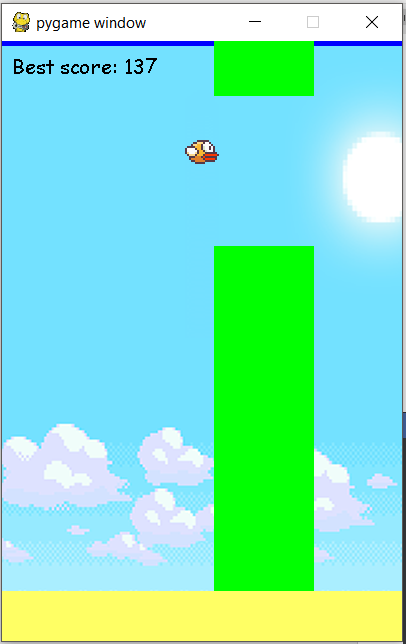
\includegraphics[width=\textwidth]{score137}
        \caption{Generation = 300, BestScore = 137}
        \label{fig:Input}
    \end{subfigure}
    ~ %add desired spacing between images, e. g. ~, \quad, \qquad, \hfill etc. 
      %(or a blank line to force the subfigure onto a new line)
    \begin{subfigure}[b]{0.2\textwidth}
        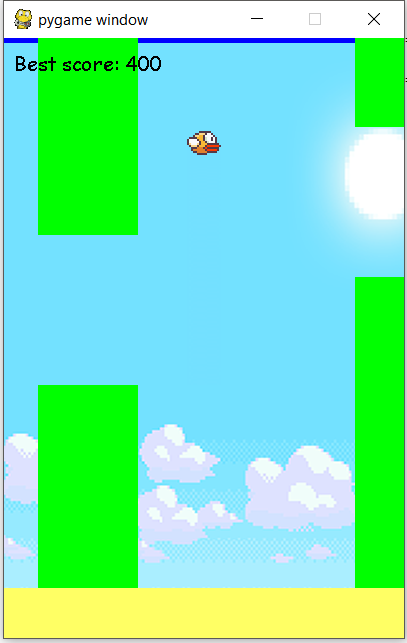
\includegraphics[width=\textwidth]{score400}
        \caption{Generation = 350, BestScore = 400}
        \label{fig:Output}
    \end{subfigure}
    \caption{Experiment result}
\end{figure}

\section{Genetic Algorithm Methodology}
\subsection{Optimization Problem}
Most problem in real life don't have formula and technique to calculate the exact result because of the vast generic complexity. GA works on a population of possible solutions and evolve them using method inspired by Darwin's theory in biology. The rest of the report will discuss the different between GA and other method and also perform some experiment to estimate the effectiveness of GA.\\
\indent
Each problem using GA requires a \textbf{fitness function} which measures the quality of the solution toward an optimization problem.
\subsection{Terminology}
In GA, a \textbf{population} of candidate solutions (also called phenotypes) is evolved toward better solutions of an optimization problem. Each candidate solution is represented by a \textbf{chromosome} which is a set of \textbf{genes} which can be alter \textbf{mutate} and \textbf{crossover}. A new set of chromosome, also known as \textbf{generation} is formed using \textbf{selection}.
\subsubsection{Population, chromosome and genome}
~\\
\textbf{Population}: The number of individuals present with same length of chromosome. In other words, they are a set of possible solution to a optimization problem.\\
\textbf{Genome}: A part of a chromosome. The value of each gene has an effect on the quality of solution.\\
\textbf{Chromosome}: A set of genomes. Chromosome is the solution in form of genes
\begin{figure}[H]
    \centering
    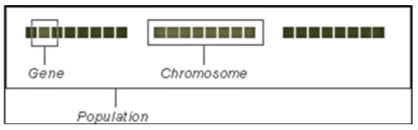
\includegraphics[width=8cm]{gene_definition}
    \caption{Population, Chromosomes and Genes}
    \label{fig:fig2}
\end{figure}
\subsubsection{Selection, mutation and crossover}
~\\
\textbf{Selection}: Next generation's population will keep some of the best solution in the previous generation so that best traits is retained.\\
\textbf{Mutation}: Alter genome in chromosome.\\
\textbf{Crossover}: Mixing two individual to produce a new pair of offspring that have the trait of both 
\section{Genetic Operators}
\subsubsection{Encoding and Decoding} \label{encode}
Encoding technique depends heavily on the problem. Generally, encoding is the order of every genes that have an effects on the solution. Decoding is translate chromosome to solution of optimization problem. Encoding is a method to clean data before putting it in genetic operators.
\begin{center}
 \begin{tabular}{||c c||} 
 \hline
 Encoding Method & Chromosome \\ 
 \hline\hline
 Binary & 1011000010010  \\ 
 \hline
 Value & 1 2 6 7 1 8 0 1 5 \\
 \hline
 Value & ABDOMNABCDAC \\
 \hline
 Value & (back), (back), (right), (forward)\\[1ex] 
 \hline
\end{tabular}
\end{center}
\subsubsection{Selection}
Selection process is mainly responsible for assuring survival of the best-fit
individuals. Best solution will be retained in the next generation.
\\
\indent
\indent
\textit{2.1) Roulette wheel selection method}
Fitness proportionate selection, also known as roulette wheel selection, is a genetic operator used in GA for selecting potentially useful solutions for recombination.\\
In this method, each gene have a probability of being selected for next generation. This probability is defined by:
\begin{equation} \label{eq:1}
p_i = \frac{f_i}{\sum_{j=1}^{N}f_j}
\end{equation}
$p_i$: Probability of individual with index $i$ being selected.\\
$f$: Fitness function\\
$f_i$: Fitness value of individual with index $i$\\
\indent
\indent
\textit{2.2) Best fitness selection method}\\
In this selection method, best individuals with highest fitness is being selected. This method is a trade off between diversity of population and average fitness of population where diversity decreases and average fitness increases in comparison with Roulette wheel selection method.
\subsubsection{Mutation}
~\\
\indent
Mutation is used to maintain genetic diversity from one generation of a population of
chromosomes to the next. It is analogous to biological mutation. \\
\indent
The purpose of mutation in GA is preserving and introducing diversity. Mutation should
allow the algorithm to escape local minima by preventing the population of chromosomes
from becoming too similar to each other, thus slowing or even stopping evolution. Mutation can be done with a formula or randomly.
\begin{figure}[H]
    \centering
    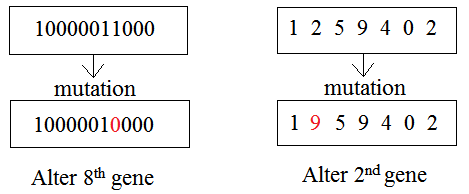
\includegraphics[width=7cm]{mutation}
    \caption{Example of mutation on binary encoding and value encoding}
    \label{fig:fig3}
\end{figure}
\subsubsection{Crossover}
~\\
\indent
The crossover splits up the parent individuals and recombines them. Crossover point can be chosen randomly to increase diversity of new population.
\begin{figure}[H]
    \centering
    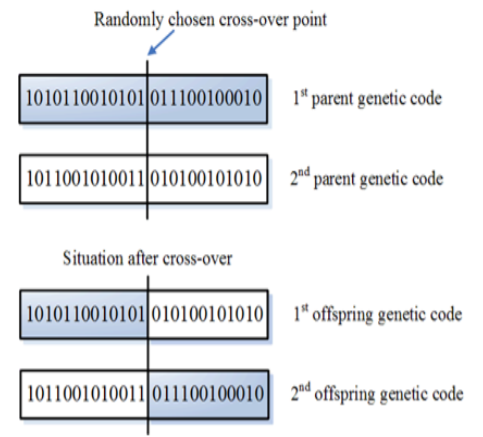
\includegraphics[width=7cm]{crossover}
    \caption{Genetic Code of the parents and offspring before and after the crossover~\cite{4}}
    \label{fig:fig4}
\end{figure}
\indent
Multi-point crossovers are simply crossovers with
more than one position where crossover will occur.

\section{Implementation}
\subsubsection{Implementation overview}
\indent The algorithm can be done by continuously create new set of possible solution using GA to evolve every generation overtime until an acceptable solution is found.\\

\subsubsection{Flowchart}
\indent
\begin{figure}[H]
    \centering
    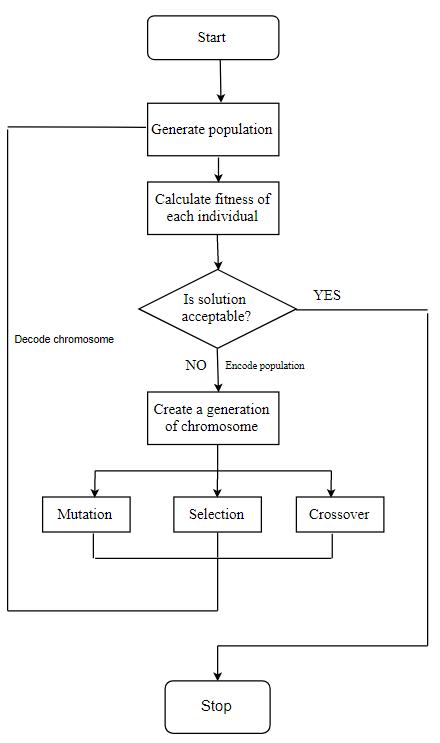
\includegraphics[width=8cm]{flowchart}
    \caption{GA Flowchart}
    \label{fig:fig5}
\end{figure}
\subsubsection{Pseudo Algorithm}
~\\
START\\ \\
Initializing population.\\
Calculate fitness of each individual.\\ \\
DO UNTIL BEST SOLUTION IS FOUND\\ \\
\indent	Encoding each individual to produce chromosome.\\
\indent Perform GA operators on exist population\\
\indent Decode new population and kill old population\\ \\
LOOP\\ \\
END\\ 
\section{Application in building AI for Flappy Bird Game}
\subsection{Gameplay overview}
Flappy Bird is a mobile game developed by a Vietnamese developer Dong Nguyen. The objective was to direct a flying bird, named "Faby", who moves continuously to the right, between sets of Mario-like pipes. If the player touches the pipes, they lose. Faby briefly flaps upward each time that the player taps the screen; if the screen is not tapped, Faby falls because of gravity; each pair of pipes that he navigates between earns the player a single point.
\subsection{Training model}
In this section, multilayer perceptron model will be discussed and an implementation on Flappy Bird game will also be provided.
\subsubsection{Neural Network Overview}
~\\
\indent \indent
$1.1)$ Layer: They are a set of neuron (a circle that contain a number). Beside input layers and output layers, one Multilayer Perceptron can have one or more hidden layer
\begin{figure}[H]
    \centering
    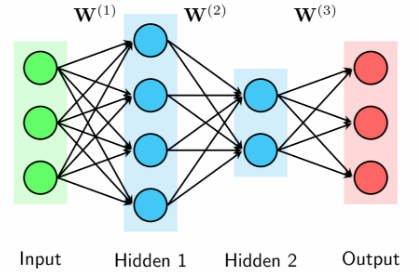
\includegraphics[width=8cm]{nnmodel}
    \caption{Example of multilayer perceptron network with 2 hidden layers}
    \label{fig:fig6}
\end{figure}
\indent \indent
$1.2)$ Unit: One node (the circle in Fig $6$) is called one unit. Input of each unit is symbolised as $z$ and output of each unit is symbolised as $a$ ($a$ stands for activation, input unit  in next layer)
~\\
\\
\indent \indent
$1.3)$ Weights and Biases: In fig $7$, the number that in the line which connects 2 nodes in 2 layer is called Weights, they determine how much affect a node could have on the next input unit in the next layer, biases is the node $x_0$ in fig 7, the value is normally constant at 1. They add the flexibility to the network.
\begin{figure}[H]
    \centering
    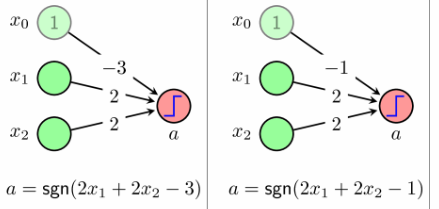
\includegraphics[width=8cm]{feedforward}
    \caption{Feed Forward Process with Sigmoid activator}
    \label{fig:figa}
\end{figure}
\indent \indent
$1.4)$ Activator, activation function: When talking about activator, they mean the function that apply on a nodes to produce the output unit. The purpose of activation function is to squeeze the value after multiplying nodes value and weights to produce a number within a defined range.
\begin{figure}[H]
    \centering
    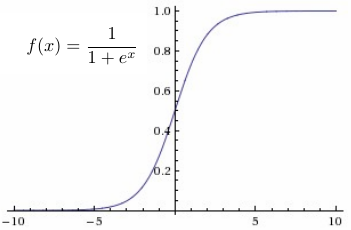
\includegraphics[width=8cm]{sigmoid}
    \caption{Sigmoid function squeeze number to value of 0 when $s$ goes to -infinity and 1 when $x$ goes to infinity}
    \label{fig:fig6}
\end{figure}

\begin{figure}[H]
    \centering
    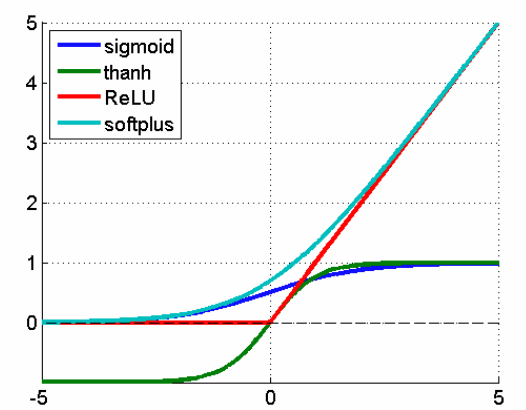
\includegraphics[width=8cm]{activator}
    \caption{Different activation functions}
    \label{fig:fig6}
\end{figure}
\subsubsection{Neural Network for Flappy Bird AI}
In this experiment, a simple multilayer perceptron model \cite{5} is chosen. The network includes one hidden layer with 6 nodes, one output layer and one input layer. One bias node is added in input layer and hidden layer. These bias nodes ensure constant variable can have an effect on the solution. Hidden layer and output layer use sigmoid function as activator.
Output of neural network is a number in range 0 and 1. Threshold is set to $0.5$. If $output>0.5$ then the bird will flap. \\
Source code can be found at: \\ $https://github.com/DungLai/AI-FlappyBird$
\begin{figure}[H]
    \centering
    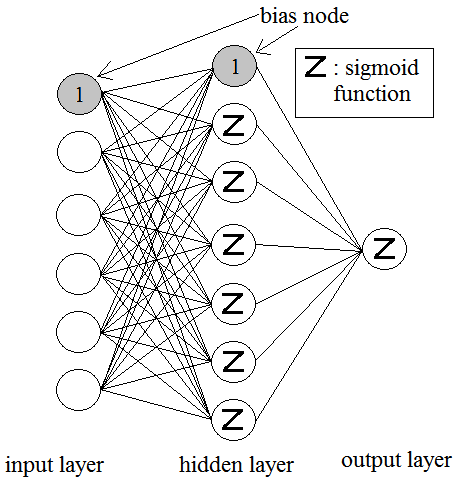
\includegraphics[width=8cm]{neural}
    \caption{Neural Network Architecture}
    \label{fig:fig6}
\end{figure}
\subsection{Input for training model}
In neural network, every input should be related to the solution. There are 5 inputs as described in figure~\ref{fig:fig6}\\
\begin{figure}[H]
    \centering
    \begin{subfigure}[b]{0.2\textwidth}
        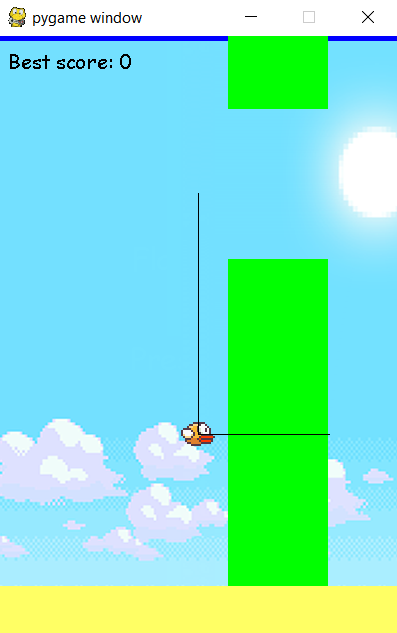
\includegraphics[width=\textwidth]{sensor}
        \caption{Two sensors of a bird horizontal line, vertical line}
        \label{fig:fig7}
    \end{subfigure}
    ~ %add desired spacing between images, e. g. ~, \quad, \qquad, \hfill etc. 
      %(or a blank line to force the subfigure onto a new line)
    \begin{subfigure}[b]{0.2\textwidth}
        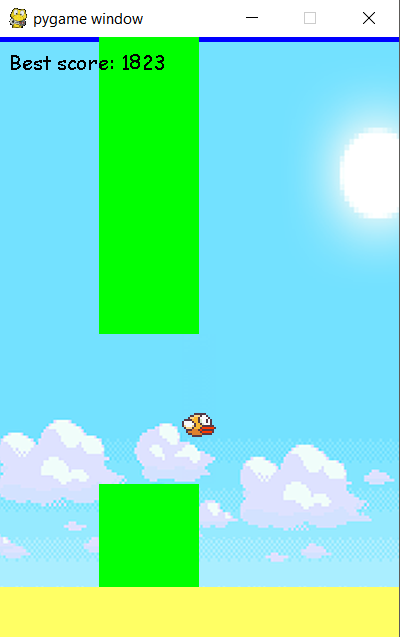
\includegraphics[width=\textwidth]{score1823}
        \caption{Best performance 1823 scores}
        \label{fig:fig7}
    \end{subfigure}
    \caption{Experiment result}
\end{figure}
\indent Input 1: Horizontal distance between bird and Tube (Horizontal line in figure~\ref{fig:fig7}).\\
\indent Input 2: Vertical distance between bird and the middle of two tubes (Vertical line in figure~\ref{fig:fig7}).\\
\indent Input 3: Width of bird.\\
\indent Input 4: Height of bird.\\
\indent Input 5: Width of tube.
\subsection{Implementation of GA}
\subsubsection{Encode}
There are 49 weights in neural network in figure~\ref{fig:fig6}. All of these weights are added into an float array of size 49. This array will carry all the information of the whole network. As a result, each array is considered as an chromosome with value encoding method (described in~\ref{encode}). Each weight is now a gene in a chromosome.
\subsubsection{Applying genetic operator}
Selection, mutation and crossover is used in this experiment.\\
Selection: Best fitness selection method (III-$2.2$)\\
Mutation: Modify a weight by randomly assign a new number to it. (III-$4$)\\
Crossover: Exchange two weight by a fixed possibility (III-$3$)\\
\begin{center}
 \begin{tabular}{||c c||} 
 \hline
 Parameter & Value\\ 
 \hline\hline
 POPULATION & 50 \\ 
 \hline\hline
 SELECTION RATE & 0.1 \\ 
 \hline\hline
 MUTATION RATE & 0.7   \\ 
 \hline
 CROSSOVER RATE & 0.6 \\
 \hline
 MUTATION PERCENTAGE & 0.6 \\
 \hline
 CROSSOVER PERCENTAGE & 0.1 \\[1ex] 
 \hline
\end{tabular}
\end{center}
\subsubsection{Fitness function}
In this experiment, fitness function is simply the survival time of a bird, the unit is the number of frames being refreshed after the bird dies.
\section{Experiment Statistical Result}
\begin{figure}[H]
    \centering
    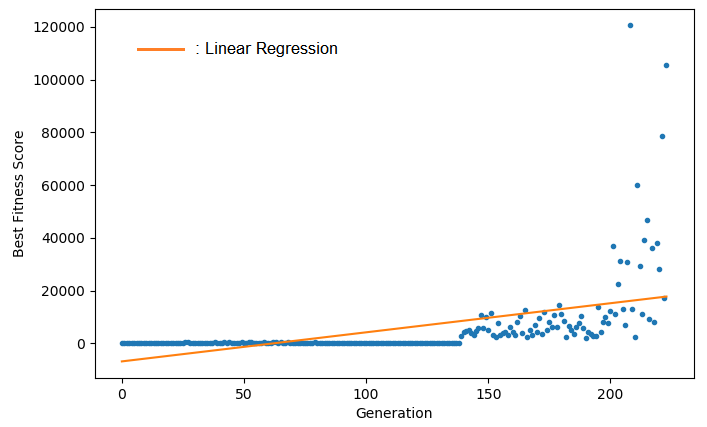
\includegraphics[width=8cm]{plot}
    \caption{Experimental result 1}
    \label{fig:fig7}
\end{figure}
\begin{figure}[H]
    \centering
    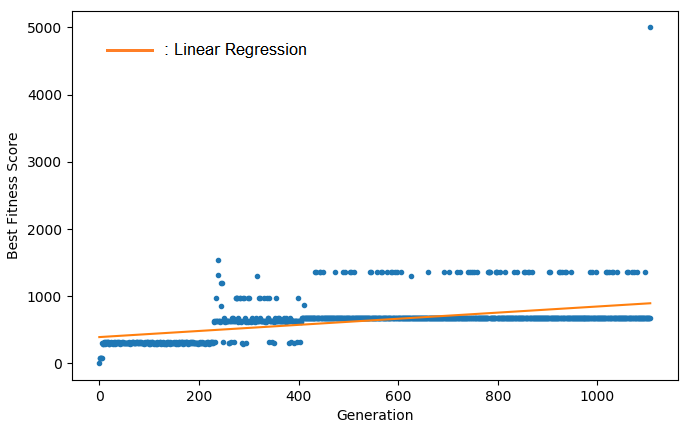
\includegraphics[width=8cm]{plot2}
    \caption{Experimental result 2}
    \label{fig:fig8}
\end{figure}
The two above graphs describe the correlation between number of generation and best fitness score to figure out if GA actually helps the population evolve over time or not. In both experiment, an impressive solution is found. However, the first experiment took 230 generations while the second experiment took over 1000 generations in order to find the best solution. A correlation coefficient (Pearson) is performed to test whether there is a correlation between number of generation and best fitness score.
\begin{center}
 \begin{tabular}{||c c c||} 
 \hline
 Experiment & pearson-r & p-value\\ 
 \hline\hline
 Experiment 1 & 0.5 & 0.001 \\ 
 \hline \hline
 Experiment 2 & 0.5 & 0.001 \\[1ex] 
 \hline
\end{tabular}
\end{center}
Both experiment share the same result, there is a strong, positive linear relationship between number of generation and best fitness score and Pearson's correlation shows that this relationship is significant, $r=.5$, $p<.001$.\\
\indent 
We can conclude that GA do improve the optimization overtime. However, time complexity cannot be measured exactly due to the high arbitrary aspect.
\section{Further Research}
\indent
As there are many randomness in GA, the experiment result could be biased. Further research can be done by controlling the arbitrary factors. 
\section{Discussion}
\indent
It can clearly be seen that there is not much concrete mathematical foundation to GA. The algorithm itself is heavily derived from biology. The performance of GA is also not being calculated or estimated, this is the reason why many people tend to have negative opinions on it. However, I strongly believe that one day, researcher will find a solid foundation and make improvement GA. Neural network is an example, the idea is derived from an unrelated field, namely neuroscience, nodes describe the connection between millions of neurons in the brain of human. Overtime, researchers and developers improve the performance of neural network, some fantastic training technique such as backpropagation are introduced and ensure the convergence of the optimization problem, many variations have been made to neural network too, such as convolutional neural network (CNN), recurrent neural network (RNN) and long short-term memory (LSTM) architecture. Again, I strongly believe that the same boom in research will happen to GA one day.
\section*{Acknowledgment}
\indent
The author would like to thank Luke Gavin, my tutor for this project. He constantly encourages me and also recommend many good pieces of advice as well as learning materials. Also thanks to Dr. Christopher McCarthy for a great serie of lecture on Object Oriented Programming (OOP), this project is part of the unit, without solid understanding of OOP, the implementation of GA as well as Flappy Bird game will be very challenging.

\begin{thebibliography}{5}

\bibitem{1}
Ali Jafari, Maryam Zekri, Saeed Sadri, Alireza Mallahzade \emph{"Design of Analog Integrated Circuits by Using Genetic Algorithm"}. [Online] Available at:
http://ieeexplore.ieee.org/document/5445763/

\bibitem{2}
Haihong Tao, Guisheng Liao, Ling Wang \emph{Space-borne antenna adaptive side-lobe nulling algorithm based on gradient-genetic algorithm.} [Online] Available at: http://ieeexplore.ieee.org/document/1321992/

\bibitem{3}
E. Eiben (1994). "Genetic algorithms with multi-parent recombination". PPSN III:
Proceedings of the International Conference on
Evolutionary Computation. The Third
Conference on Parallel Problem Solving from
Nature: 78–87. ISBN 3-540-58484-6

\bibitem{4}
E. Schultz, J. Mellander, C. Endorf (2008), "Intrusion Detection and Prevention - A basic genetic algorithm", [image online], http://my.opera.com/blu3c4t/blog/show.dml/26
36486. 

\bibitem{5}
Andrew, Ng. , 'Machine learning', Standford University Online, lecture notes week 4, [online]: https://www.coursera.org/learn/machine-learning
\end{thebibliography}

\end{document}


